\documentclass[10pt,a4paper]{article}
\usepackage{graphicx,float}
\usepackage{cite}
\usepackage{url}

\title{\LARGE
    Project Phase 1: A Detailed Analysis of SUPERCOP on the Dragonboard APQ8060.
}

\author{\large
{\bf Kevin Burns, Robert Lyerly, Reese Moore, Philip Kobezak}\\ 
Virginia Polytechnic Institute \& State University\\
1185 Perry Street, Blacksburg VA\\
\vspace{8mm}
\{kevinpb, rlyerly, ram, pkobezak\}$@$vt.edu\\
}
\date{}

\begin{document}

\maketitle


% INTRODUCTION   
%--------------
% Contains:
%   - a brief overview of the APQ8060 architecture.
%   - how we approached the problem
%   - how we partitioned the tasks
%   - how we automated the profiling
\section{Introduction}
Computers are a ubiquitous part of our society.  As computers become increasingly connected, more of our daily lives are becoming digitized.  As such, it is important that we find new ways to ensure security and privacy.  The field of Cryptography involves designing algorithms and protocols as a means of ensuring services interact with each other in a secure, private way.  Traditionally, cryptographic theory was used to develop algorithms that were highly efficient and very secure on large desktop CPUs.  However, with the dawn of mobile computing there is an increased need for power-aware cryptography.  Research in this field seeks to strike a balance, searching for algorithms that can be used in low-power settings while still being strong and secure.  New cryptographic algorithms must be evaluated on a wide variety of hardware platforms to understand how they perform in practice.

Hash functions play an important part in cryptography.  They are heavily used for authentication and digital signing, two components of cryptography that are necessary for information security.  Designing a good hash function is a complex task - the algorithm must have several characteristics such as uniformity, efficiency and infeasibility of reversing the hash.  The National Institute of Standards and Technology (NIST) is responsible for maintaining many cryptographic algorithms, including hash functions.  NIST recently held a competition to generate an alternative to SHA-1 and MD5 because of known attacks for these hash functions.  Many different researchers submitted implementations to the competitions, and the Keccak algorithm was chosen as the official implementation for SHA-3 on October 2, 2012.  However, the software hosted at http://bench.cr.yp.to contains all the SHA-3 implementations submitted to NIST so that anybody may test them.  In the first phase of our project, we were tasked with benchmarking these submissions.

\subsection{Hardware Overview}
Our platform for the first phase of the project was a Snapdragon S3 APQ8060-based Dragonboard, used for prototyping and developing for the Android platform (hereafter referred to as ``the Dragonboard'').  The Dragonboard implements a complete wireless phone system, including a wireless RF card, a sensor card (with accelerometer and gyroscope) and a touchscreen.  The Snapdragon S3 APQ8060 contains several cores for computation and processing:

\begin{enumerate}
	\item ARM1136J-S 384 MHz embedded microprocessor
	\item Qualcomm dual-core Scorpion microprocessor (up to 1.7 GHz), which has the ARM NEON SIMD extensions
	\item Qualcomm QDSP6000 and QDSP4000 DSP cores
	\item ARM7 resource and power management microprocessor
	\item Adreno 220 GPU
\end{enumerate}

Most compute-intensive tasks are run on the larger Scorpion cores (which are designated as ``application cores''), the QDSP6000 DSP and the Adreno 220 GPU.  The ARMv7 instruction set architecture (ISA) is the 7th-generation of the ARM ISA.  It is a RISC ISA and contains a standardized 3-stage pipeline (although implementations may contain longer pipelines) and 16 x 32-bit registers.  ARMv7 also defines the NEON SIMD extensions which specify the interface to a 128-bit SIMD core with an independent pipeline and register file.  It can perform basic arithmetic and logic operations on varying size data types, including signed/unsigned 8-bit, 16-bit, 32-bit or 64-bit words.  The QDSP6000 (or ``Hexagon'') DSP is a programmable DSP designed for application use.  It has several features which make it a flexible platform, including symmetric multi-processing and VLIW/SIMD instructions (in fact, Linux has been ported to run on the Hexagon).  The Adreno 220 GPU is used for 2D and 3D rendering on Android.  It implements several graphic APIs and can be used concurrently by several of the other cores for interleaving CPU, DSP and graphics operations.

\subsection{Problem Statement}
The objective of the first phase of the project was to do a detailed performance profiling for a set of hash algorithms provided by the SUPERCOP testsuite. The analyses should try to determine why each algorithm implementation excelled, compared to other implementations,  on the target platform (Dragonboard APQ8060).   

\subsection{Partitioning}
This project presented us with a large problem set that would be impossible for
any of us to do individually in the time constraints provided. This is not an
insurmountable problem because of the parallel nature of analyzing the
performance of the various algorithms. 

In order to make analyzing the various algorithms possible, we partitioned the
algorithms up between us. 


\subsection{Profiling}
A large portion of this project is profiling the various algorithms and
implementations so that we would have data to analyze. Clearly it would be
practically infeasible to do all of the performance testing by hand, as that
would involve running several hundred algorithms, and then determining which one
is the best before doing the analysis. This would have involved a great amount
of work, not only between coordinating access to the board, but also
determining how to compile any given algorithm.

Fortunately the algorithms were distributed in a performance profiling toolkit
called SUPERCOP. As we had set up a Debian chroot on the Dragonboard, and
therefore had a fully functional GNU/Linux userland and compilation environment,
it was possible to run the SUPERCOP suite. We however did not need to run the
entire suite of tools, nor did we need to run the entire gamut of compilers and
optimizers, so in an effort to make the tests more efficient, we modified the
toolkit to better suit it to our needs. We removed a large number of compilers
that never made the official SUPERCOP list, and removed any and all algorithms
and benchmarks that would not be necessary for us to run. We also modified the
timeout so that algorithms could no hang for an hour at a time, given that we
were aiming to test the fastest algorithm.

By electing to use an automated method rather than doing the profiling by hand,
we increased our throughput by eliminating wait times between runs as well as
time when we would need to be asleep. Further this allowed us to begin
considering analysis once we had extracted partial data. The SUPERCOP scripts
allowed us to automate not only the testing but the determination of the best
algorithm. Automation of the profiling was key in completing the project in a
timely manner.




% ALGORITHMS
%------------
% Each subsection will contain:
%   - a figure containg the graph of the performance
%   - an analysis of the graph
\section{Algorithms}
\subsection{blake}
The BLAKE hash function is based on the ChaCha stream cipher, with an additional XOR each round. The way it works is,
the ChaCha algorithm works with a 4 by 4 array of words. BLAKE combines an 8-word hash value with 16 words from the 
message repeatedly, in turn truncating the ChaCha result to obtain the next hash value.The BLAKE hash function has two variants, 
a variant with a word size of 32 bits and a variant with a word size of 64 bits. The first two hash functions we evaluate, blake32 and blake256, are 
of the 32 bit word variety.

\subsubsection{blake32}
\begin{figure}[H]
    \begin{center}
        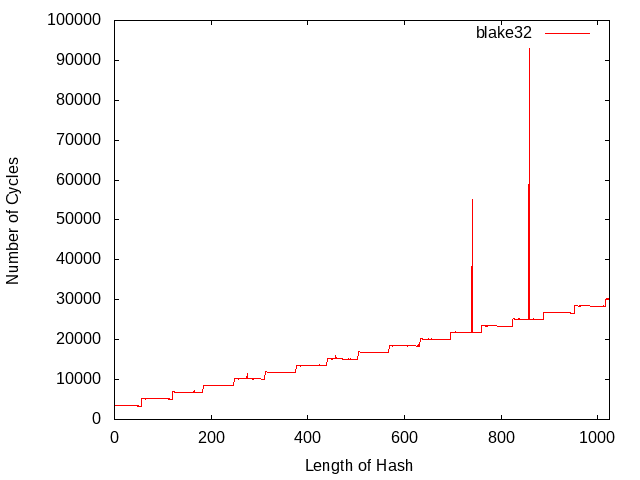
\includegraphics[scale=0.5]{images_fast_run/blake32.png} 
        \caption{BLAKE with 32-bit words, 10 rounds, and 256-bit output}
    \end{center}
\end{figure}

From the graph above we see that there is a stepwise characteristic. The steps seem to increment every time the hash is divisible by 64. 
This characteristic is present due to the fact that during each iteration 2 words are taken from the message at one time. So a total of 64 bits
of the actual message is processed. This happens 8 times a round, therefore 512-bits are processed per round. So, as our hash size increases by 
multiples of 64 bytes we will see more and more iterations having to be processed.

\subsubsection{blake256}
    \begin{figure}[H]
        \begin{center}
            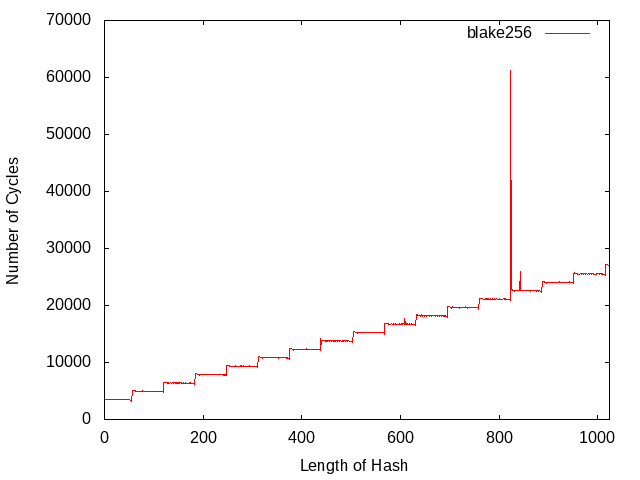
\includegraphics[scale=0.5]{images_fast_run/blake256.png} 
            \caption{BLAKE with 32-bit words, 14 rounds, and 256-bit output}
        \end{center}
    \end{figure}

The graph above shows a very similar pattern to the blake32 graph. The reason is that blake256 also uses a 32 bit word size. The difference we
see between the blake32 and this graph is the number of cycles. When analyzing the data I found that the cycles per byte for blake32 was twice
that of blake256. This seems counter intuitive as blake256 has an additional 4 rounds to compute each iteration. I speculate that this is
due to the compiler options chosen by the script we ran to find the fastest implementation of each algorithm. The options chosen for blake256 were 
(compiler gcc -mcpu=arm1136jf-s -O -fomit-frame-pointer -fno-schedule-insns 4.4.5) versus the options for blake32 
(gcc -mcpu=arm9tdmi -O2 -fomit-frame-pointer 4.4.5). As we can see the architecture chosen by the script is not the target architecture and could
lead to a number of mis-optimizations. 

\subsubsection{blake64}
    \begin{figure}[H]
        \begin{center}
            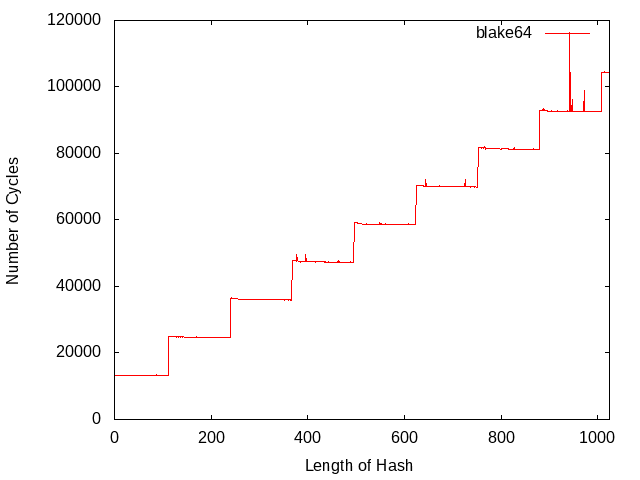
\includegraphics[scale=0.5]{images_fast_run/blake64.png} 
            \caption{BLAKE with 64-bit words, 14 rounds, and 512-bit output }
        \end{center}
    \end{figure}
The blake64 hashing function increases the word size to 64 bits. Since nothing else changes we see that the widths of each step in our 
stepwise graph is doubled, so 1024 bits long. The cycles per byte were higher than that of the 32-bit word sizes. This is due to the 
fact that the target processor is a 32 bit architecture and does therefore doesn't have a chance to utilize 64 bit words. 

\subsubsection{blake512}
    \begin{figure}[H]
        \begin{center}
            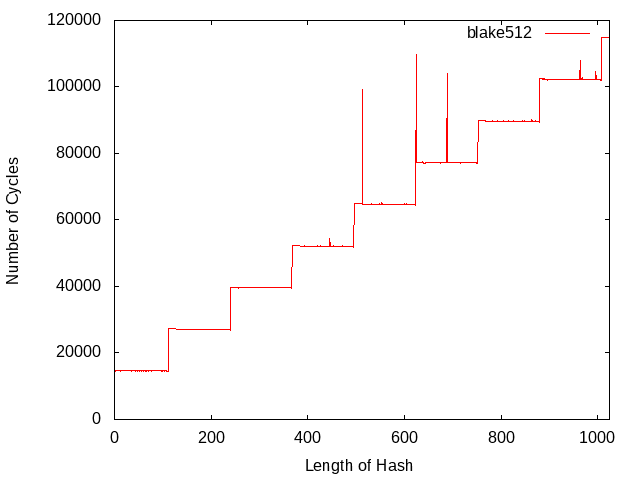
\includegraphics[scale=0.5]{images_fast_run/blake512.png} 
            \caption{BLAKE with 64-bit words, 16 rounds, and 512-bit output}
        \end{center}
    \end{figure}
The difference between blake512 and blake64 is the number of rounds. This would explain the identical step width, 128 bytes, along with the increase
in cycles for blake512. 

\subsection{cubehash}
I won't explain the details of cubehash here. I will instead talk about how the choice of variable sizes in the cube hash equation is reflected on the graph, along with the possible influence from the architecture. If we represent the equation as CubeHashi+r/b+f–h(m). Where i is the number of initialization rounds, r is the number of rounds per message block, b is the length of the blocks taken from the message, f is the number finalization rounds, h is the number of output bits, and m is the message. We're given that r is 8 rounds per block, b is 16 bytes in a block, and h is 512 bits of output.
\subsubsection{cubehash816}
    \begin{figure}[H]
        \begin{center}
            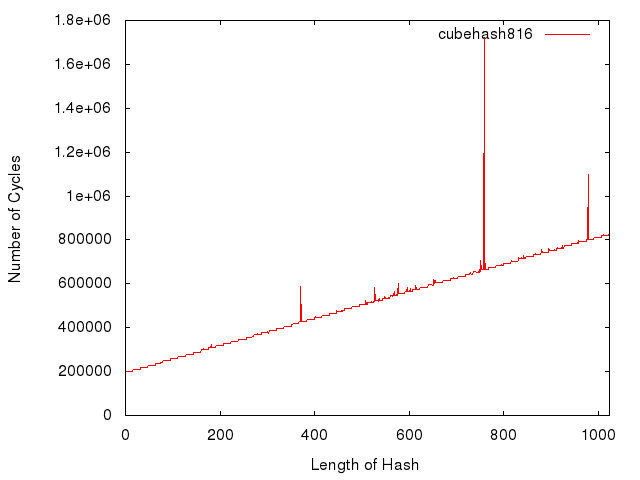
\includegraphics[scale=0.5]{images/cubehash816.png} 
            \caption{CubeHash8/16 with 512-bit output}
        \end{center}
    \end{figure}

The implementation selected for benchmarking was the simple implementation,
compiled using \texttt{gcc -mcpu=arm8 -Os -fomit-frame-pointer} using GCC
version 4.4.5.

It is a little hard to see in the above graph, but it takes on a similar shape to the graphs found in the blake algorithms. That is, it is as step like characteristics. The length of each step is 16 bytes, 128 bits. This appears to be from the size of the blocks processed each round. Each block is 16 bytes as described above. When the message increments by a multiple of 16 we see a rise in the step. As that's one more block that needs to be processed.  
Our target platform can provide 16, 32bit registers for the processing each block. This may be a responsible for the given speed.

\subsection{groestl}
The groestl algorithm is another block cipher that is based from AES. This function works with l-bit blocks where l is 2n and n is the number of output bits. In this case n is 256 and 512 as denoted in the names. 

\subsubsection{groestl256}
    \begin{figure}[H]
        \begin{center}
            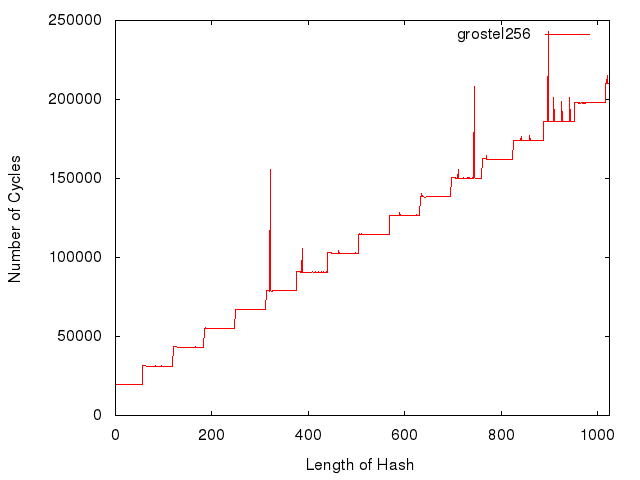
\includegraphics[scale=0.5]{images/grostel256.png} 
            \caption{Gr{\o}stl with 256-bit output}
        \end{center}
    \end{figure}

The implementation selected for benchmarking grostel256 is the 32bit-2ktable
implementation compiled using \texttt{gcc -mcpu=arm7tdmi -O3
-fomit-frame-pointer} on GCC version 4.4.5. The selection of a 32 bit
optimization makes sense given that we are targeting a 32 bit platform. A table
based implementation implies that the memory tradeoff versus calculation was a
preferable implementation decision.

The graph above also shares the step like characteristics of the other graphs. Each step for this plot is 64 bytes, 512 bits in length. From what we know about groestl, it works with l-bit blocks, where we derived above l is 512 bits. We can then correlate this to the nature of the step size witnessed in the graph above.

\subsubsection{groestl512}
    \begin{figure}[H]
        \begin{center}
            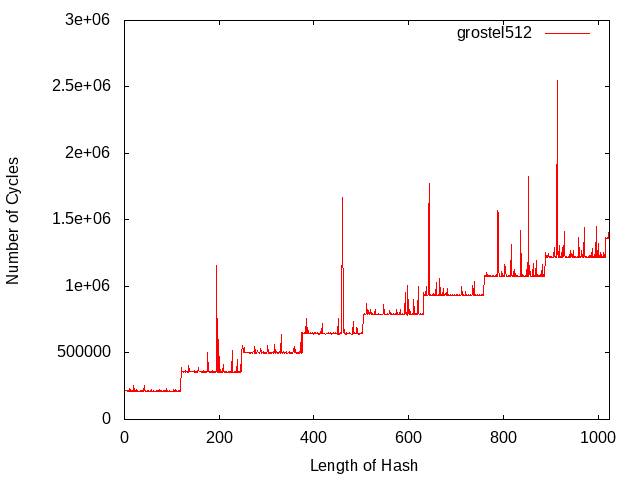
\includegraphics[scale=0.5]{images/grostel512.png} 
            \caption{Gr{\o}stl with 512-bit output}
        \end{center}
    \end{figure}

The implementation used to benchmark grostel512 was the 32bit-bytesliced-c-small
1.0 compiled using \texttt{gcc -mcpu=strongarm110 -O -fomit-frame-pointer} on
GCC version 4.4.5. Again, the selection of a 32 bit optimized version for a 32
bit platform is an obvious performance enhancing decision. Further, the
selection of byteslicing shows that that is an effective speedup mechanism
compared to other grostel512 implementations.

This graph shows performance severely degraded from groestl256.  First, we note that since the digest size is 512 bits, the block size is 1024 bits (or 128 bytes), which corresponds to the step size portrayed in the graph.  However there are several additional sources of overhead that make this implementation slower.  First, this version of the algorithm performs 4 additional rounds (14 rounds versus the 10 performed in groestl256).  Also, there is a difference in the round calculations.  Gr{\o}stel-256 performs operations on 8x8 matrices of bytes whereas Gr{\o}stel-512 operates on 8x16 matrices of bytes.  The added extra columns manifests themselves in an order of magnitude difference between the performance of the two algorithms.  Because the operations can no longer be broken down into clean 32-bit operations, the algorithm suffers a massive penalty.

\subsection{JH}
%%%
% Some general discussion about the JH functions that we're gonna reference
% later.
%%%
The JH family of hash functions are a set of functions that were submitted to
the NIST SHA-3 competition. The submission defines four specific hash
algorithms: JH-224, JH-256, JH-384, and JH-512. All of these separate functions
are implemented through a very similar construction, and as such one would
expect them to exhibit similar performance properties as well as optimization
opportunities.

Wu\cite{wu2008jh} describes the hash function family in his submission to the
NIST competition. JH is constructed through a simple to describe compression
function that is shared by all variants. The compression function maintains
$1024$ bits of internal state and operates on $512$ bit blocks at a time. Even
before doing performance analysis, this would indicate that we should expect to
see a jump in the number of cycles required every $64$ bytes, as at those byte
boundaries the function has to process another block of data. The differences
between the functions are in how the context of the hash is seeded and how much
of the data is taken off the end to form the digest, and so we would expect to
see similar performance across all of the JH functions.

%%%
% The JH-224 Variant.
%%%
\subsubsection{JH-224}
\begin{figure}[H]
    \begin{center}
        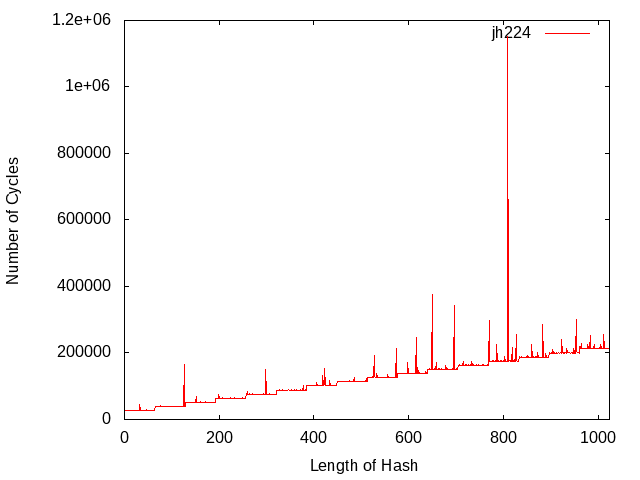
\includegraphics[scale=0.5]{images/jh224.png} 
        \caption{JH-224 with 224-bit output}
    \end{center}
\end{figure}

The algorithm selected for benchmarking JH-224 was bitslice\_opt32 compiled with
\texttt{gcc -mcpu=arm920t -O2 -fomit-frame-pointer} with GCC version 4.4.5. This
choice makes sense given the 32 bit word length of this Snapdragon processor,
and the fact that JH is designed such that bitslicing is an effective
optimization technique\cite{wu2008jh}. 

We note that the prediction that there would be a jump in the number of cycles
used every $64$ bytes was confirmed. We further note that each jump appears to
be roughly equivalent, implying that they are attributable to similar phenomena,
further confirming our suspicions. 

Wu\cite{wu2008jh} gives details about the bit-slicing implementation used for
JH. The implementation he defines performs bit-slicing optimizations on
components of the 512-bit block used in the encryption permutation, and leaves
the overall construction largely unaffected. This explains why we still see the
$64$ byte block boundaries playing an important roll in defining the shape of
the performance graph.


%%%
% The JH-256 Variant.
%%%
\subsubsection{JH-256}
\begin{figure}[H]
    \begin{center}
        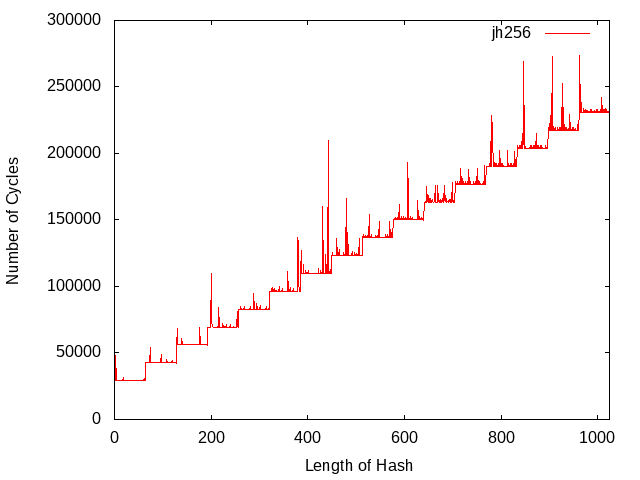
\includegraphics[scale=0.5]{images/jh256.png} 
        \caption{JH-256 with 256-bit output}
    \end{center}
\end{figure}

The algorithm selected for benchmarking JH-256 was bitslice\_opt32 compiled with
\texttt{gcc -mcpu=arm8 -O3 -fomit-frame-pointer} with GCC version 4.4.5. Again,
this choice of algorithm makes sense given that the Snapdragon processor has a
32 bit word length. Interestingly, different optimization options were selected
during the profiling process for JH-256 than for JH-224, however this would lead
us to believe that this implementation is designed in such a way that the
compiler is not given enough leeway to make meaningful optimizations based on
the differences.

We again note that our predicted graph shape held, and that the growth of this
function is roughly similar to that of JH-224. This is what we would expect
given that all variants of JH share a compression function.


%%%
% The JH-384 Variant.
%%%
\subsubsection{JH-384}
\begin{figure}[H]
    \begin{center}
        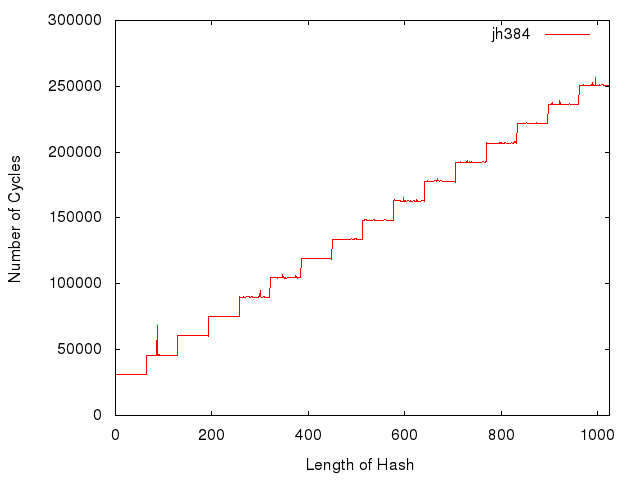
\includegraphics[scale=0.5]{images/jh384.png} 
        \caption{JH-384 with 384-bit output}
    \end{center}
\end{figure}


%%%
% The JH-512 Variant.
%%%
\subsubsection{JH-512}
\begin{figure}[H]
    \begin{center}
        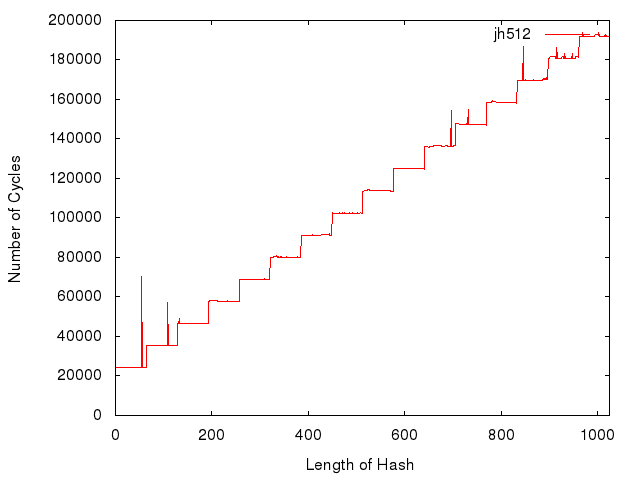
\includegraphics[scale=0.5]{images/jh512.png} 
        \caption{JH-512 with 512-bit output}
    \end{center}
\end{figure}

The algorithm selected for benchmarking JH-512 was bitslice\_opt32 compiled with
\texttt{gcc -mcpu=cortex-a9 -mfloat-abi=softfp -mfpu=neon -Os -fomit- \\
frame-pointer} with GCC version 4.4.5. This optimized algorithm makes sense for
the 32 bit Snapdragon processor, and given that JH is easily optimized through
bit-slicing. In this instance we have a different set of optimization
parameters, we do note a slight drop in the cycles consumed at the high levels
so perhaps optimization for the NEON FPU is beneficial or optimization for size
allows better management of the cache. Regardless, the performance graph is very
similar to the other graphs both in size and growth rate, and this can be
attributed to the shared compression function used across all lengths of JH.

\subsection{Keccak}
Keccak is an entry into the NIST SHA-3 cryptographic hash competition, and
ultimately was chosen by NIST to become SHA-3. Keccak describes a family of
cryptographic hash functions designed as a sponge construction. Bertoni et al.\
describe Keccak in \cite{bertoni2009keccak}. They build the specific variants of
Keccak on top of a permutation function called Keccak-f[b].

Variants of Keccak are primarily defined by three security parameters: the width
of the Keccak-f permutation: $b$, the capacity (the probability of success for
any generic attack against a sponge construction): $c$, and the number of rounds in
Keccak-f: $n_r$\cite{bertoni2009keccak}. The choice of these parameters has an
effect not only on the security level of the Keccak variant, but also the
performance. $r$ defines the bitrate of the sponge function, that is to say how
many bits the sponge function processes at a time, and accordingly how many
calls to the Keccak-f function are going to be made for a bitstring of a given
length. Therefore, the $r$ value is directly proportional to what we should see
as the length between upward steps in the number of cycles required to process
data.

Interestingly, the designers say that although Keccak-f is standardized on
having a width of $1600$ bits, this is optimized for a 64 bit processor. They
suggest that users of 32 bit and even embedded processors tune the function to
have a smaller width, such as $800$ to obtain better performance without totally
sacrificing security\cite{bertoni2009keccak}.

\subsubsection{keccak}
\begin{figure}[H]
    \begin{center}
        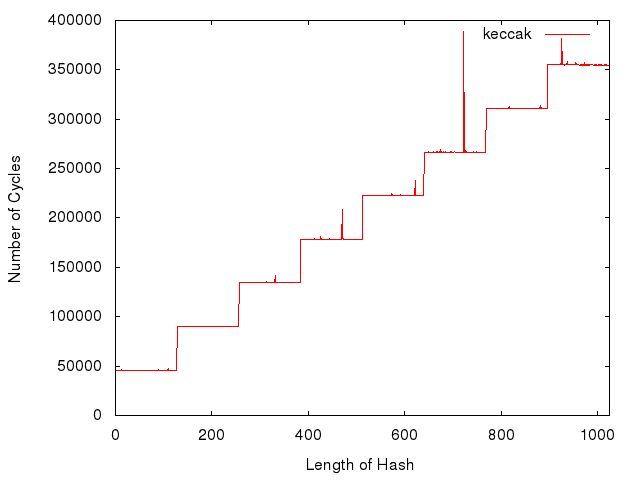
\includegraphics[scale=0.5]{images/keccak.png} 
        \caption{Keccak[]=Keccak[r=1024,c=576,nr=24] with 1024-bit output}
    \end{center}
\end{figure}

The algorithm selected to benchmark Keccak was compact, which had been compiled
with \texttt{gcc -funroll-loops -O -fomit-frame-pointer} with GCC version 4.4.5.
This version of Keccak has the parameters $ r = 1024, c = 576, n_r = 24$.

We note the stair stepped function that we associate with an additional call to
the underlying Keccak-f permutation function. We note that the steps occur every
128 bytes, which is in line with our assumption that they would be defined by
the bitrate $r = 1024$. 


\subsubsection{keccakc256}
\begin{figure}[H]
    \begin{center}
        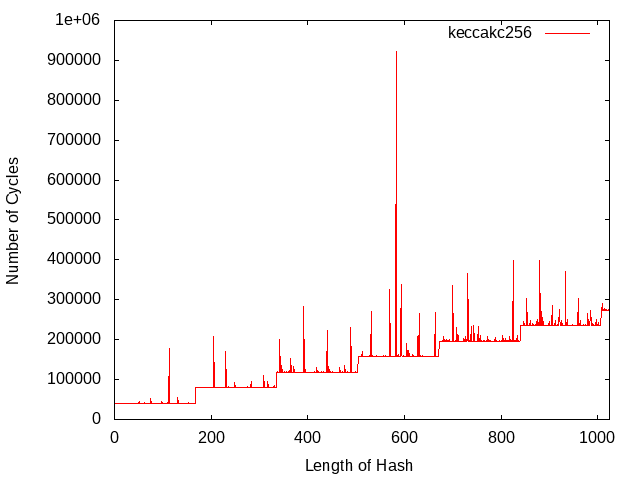
\includegraphics[scale=0.5]{images/keccakc256.png} 
        \caption{Keccak[r=1344,c=256,nr=24] with 1344-bit output}
    \end{center}
\end{figure}

The algorithm selected to benchmark Keccakc256 was compact, which had been
compiled with \texttt{gcc -mcpu=cortex-r4 -O2 -fomit-frame-pointer} with GCC
version 4.4.5. This variant of Keccak has the parameters $r=1344,c=256,n_r=24$.


This is the same implementation style as Keccak, which is unsurprising given
that all versions of Keccak are built on a similar construction. Additionally,
this version of Keccak has similar parameters to Keccak above. The longer
bit rate correctly predicts the longer period between steps on the graph when
compared to the above implementation of Keccak


\subsubsection{keccakc448}
\begin{figure}[H]
    \begin{center}
        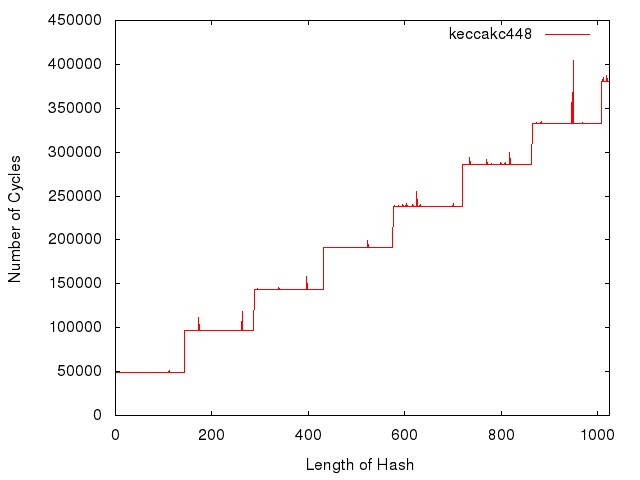
\includegraphics[scale=0.5]{images/keccakc448.png} 
        \caption{Keccak[r=1152,c=448,nr=24] with 224-bit output}
    \end{center}
\end{figure}

The algorithm selected to benchmark Keccakc448 was compact, which had been
compiled with \texttt{gcc -Os -fomit-frame-pointer} with GCC version 4.4.5. This
variant of Keccak has the parameters $r=1152,c=448,n_r=24$.

Unsurprisingly, this variant of Keccak uses the same implementation as the other
variants studied so far. This is because the Keccak family uses the same
construction internally, so optimizations from one variant for a particular
processor will work fairly well on another. 

This run shows the stair stepped pattern as well, but it is a shorter period
between the steps. This is a result of the lower bit rate of this variant.


\subsubsection{keccakc512}
\begin{figure}[H]
    \begin{center}
        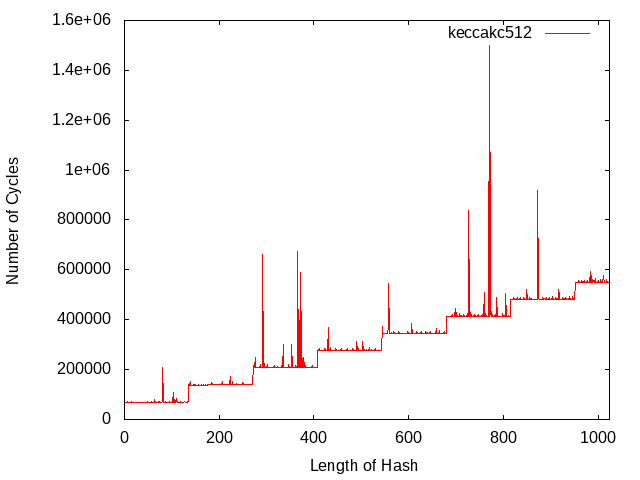
\includegraphics[scale=0.5]{images/keccakc512.png} 
        \caption{Keccak[r=1088,c=512,nr=24] with 256-bit output}
    \end{center}
\end{figure}

The algorithm selected to benchmark Keccakc512 was compact8 which had been
compiled with \texttt{gcc -mcpu=strongarm1100 -O3 -fomit-frame-pointer} on GCC
version 4.4.5. This variant of Keccak has the parameters $r=1088,c=512,n_r=24$.

Interestingly, this implementation is not what the other implementations had
been compiled with, though it is a similar implementation.

The prediction regarding the stair stepped pattern as well as the period between
the steps being proportional to the bit rate however was upheld regardless of
the differences in version. This is because the amount of work being done is
somewhat inherent in the algorithm, and these implementations are very similar.


\subsubsection{keccakc768}
\begin{figure}[H]
    \begin{center}
        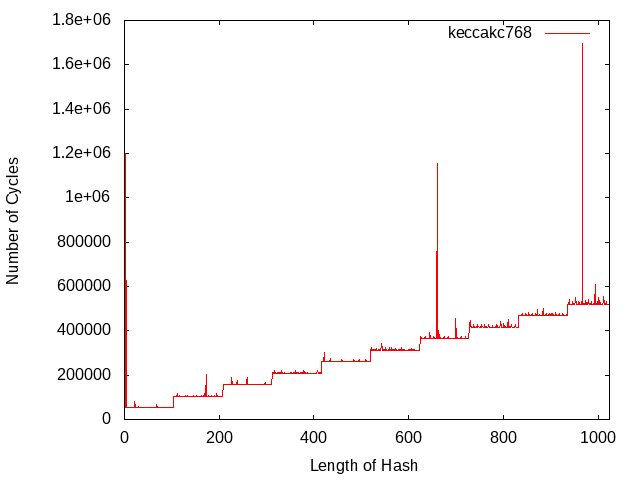
\includegraphics[scale=0.5]{images/keccakc768.png} 
        \caption{Keccak[r=832,c=768,nr=24] with 384-bit output}
    \end{center}
\end{figure}

The algorithm selected to benchmark Keccakc768 was compact which had been
compiled with \texttt{gcc -mcpu=strongarm1100 -O -fomit-frame-pointer} on GCC
version 4.4.5. This variant of Keccak has the parameters $r=832,c=768,n_r=24$.

A return to implementations of Keccak being compiled with compact on this board,
this run exhibited the exact same properties that we have been seeing before.
The stepped pattern is now shorter still because of the direct correlation with
the bit rate $r$. This performance property is a property of the algorithm
family.


\subsubsection{keccakc1024}
\begin{figure}[H]
    \begin{center}
        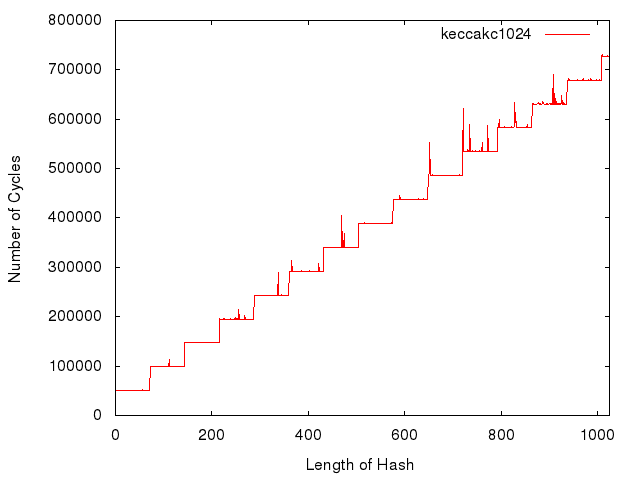
\includegraphics[scale=0.5]{images/keccakc1024.png} 
        \caption{Keccak[r=576,c=1024,nr=24] with 512-bit output}
    \end{center}
\end{figure}

The algorithm selected to benchmark Keccakc1024 was compact which had been
compiled with \texttt{gcc -mcpu=cortex-a8 -mfloat-abi=softfp -mfpu=neon -O
-fomit-frame-pointer} on GCC version 4.4.5. This variant of Keccak has the
parameters $r=576,c=1024,n_r=24$.

The version of Keccak with the shortest bit rate that we tested, and it still
upholds the prediction that the bit rate is directly correlated with the period
between the steps. In this variant, the jumps in cycle count is very rapid,
causing the algorithm to consume a much higher number of clock cycles by the
time it has finished compared to the lower capacity variants of Keccak.


\subsection{md5}
\begin{figure}[H]
    \begin{center}
        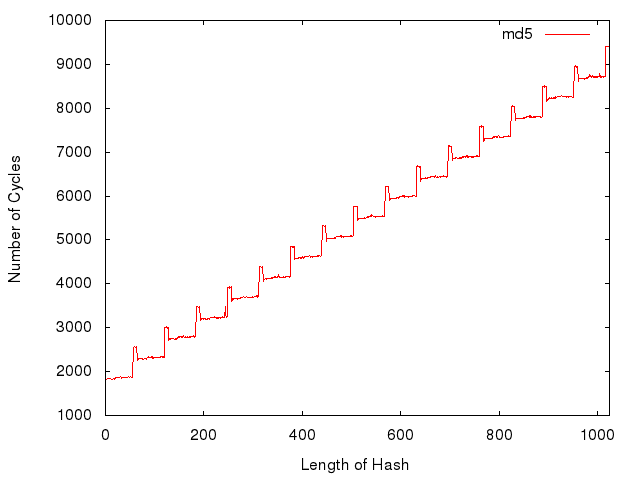
\includegraphics[scale=0.5]{images/md5.png} 
        \caption{MD5 with 128-bit output}
    \end{center}
\end{figure}


\subsection{mgr{\o}stl256}
\begin{figure}[H]
    \begin{center}
        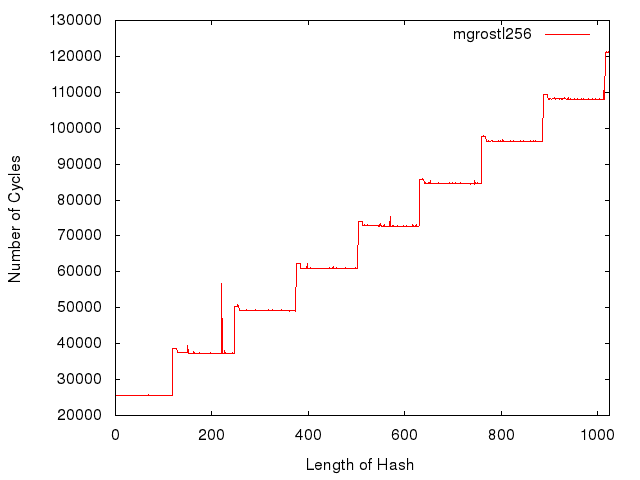
\includegraphics[scale=0.5]{images/mgrostl256.png} 
        \caption{Modifided-Gr{\o}stl with 256-bit output}
    \end{center}
\end{figure}

The modified-Gr{\o}stl (mgr{\o}stl) algorithm is a modification of the Gr{\o}stl
hash algorithm chosen as one of the five finalists of the SHA-3 competition.
Similar to other hash algorithms, an arbitrary length input is padded so that it
can be divided into 1024-bit blocks.  The algorithm works by performing a
compression function on each block; the compression function involves additions
and permutations that reduces the 1024-bit input to a 512-bit intermediate hash.
The output from each of these compression operations serves as input to the next
block with a final reduction that shrinks the message to a digest size of 256
bits. 

The implementation of mgr{\o}stl that was chosen was the opt-32 implementation
compiled with \texttt{gcc -mcpu=arm1136jf-s -O3 -fomit-frame-pointer} on GCC
version 4.4.5. The selection of a 32 bit optimized implementation makes sense
for targeting the 32 bit Snapdragon processor.

One can see the evidence of the 1024-bit block working space by looking at the
above graph. At each 128 byte boundary we see a jump in the number of cycles
that are required to perform the hashing. This is because we are doing another
complete round of the hash function on additional data.


\subsection{SHA-2}
The sha256 and sha512 algorithms are specific implementations of the previous generation SHA-2 hash function defined by NIST.  After effective attacks were found on SHA-1, NIST moved to a better hash algorithm, one which features several improvements (including fewer collisions and no known effective attacks).  Four variants of the algorithms were standardized based on the number of bits produced in the digest (including 256 and 512 bits for sha256 and sha512, respectively).

\subsubsection{sha256}
    \begin{figure}[H]
        \begin{center}
            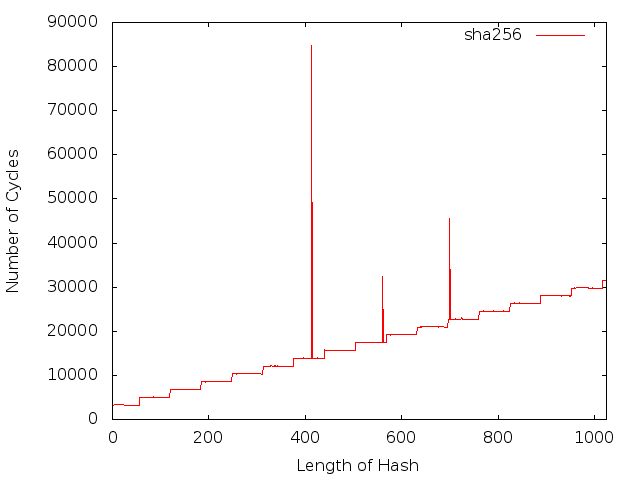
\includegraphics[scale=0.5]{images/sha256.png} 
            \caption{SHA-2 with 256-bit output}
        \end{center}
    \end{figure}

The first algorithm, sha256, works by chopping a message into 512-bit blocks and hashing each block down to 256-bits before continuing on to the next.  The result of entire hash function is added together with the original hash value, producing the final digest.  As is evident from the graph, performance models a step function with a step size of 64 bytes.  The number of blocks needed to represent the message is $\lceil$message length$/ 64 \rceil$ (this converts the number of block into an integer multiple of 64).  As soon as the message requires a higher multiple of 64 bytes, the algorithm must process another block of data.  Therefore, for every additional 64 bytes of data, another additional 64 rounds of SHA-2 must be performed.

\subsubsection{sha512}
    \begin{figure}[H]
        \begin{center}
            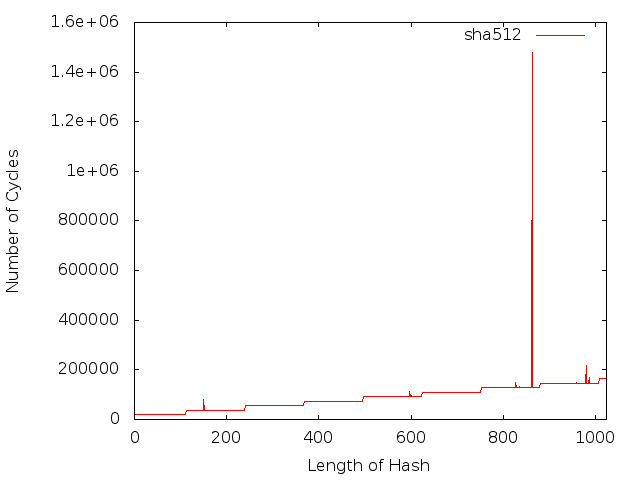
\includegraphics[scale=0.5]{images/sha512.png} 
            \caption{SHA-2 with 512-bit output}
        \end{center}
    \end{figure}

The second SHA-2 algorithm benchmarked, sha512, again produces a step function; closer inspection reveals this graph has slightly different characteristics than the one produced by running sha256.  There are some fundamental changes in the underlying algorithm - first, the digest length is 512-bits and the block size is 1024 bits.  This means that for every additional 128 bytes needed to represent the message, the algorithm must process an extra block of data - hence the step size of 128 bytes.  Because this block length is longer the algorithm must perform more calculations per round, leading to a higher cycles per byte.  Additionally, sha512 performs 80 rounds versus the 64 performed by sha256, leading to another increase in cycle count.

\subsection{Skein Hash Functions}
The Skein family of hash functions were submitted to the competition by a varied group of individuals and was one of the five finalists for SHA-3.  The Skein hash functions are based on a tweakable block cipher, named the Threefish block cipher.  The Threefish block cipher favors more rounds versus higher complexity; it only performs XOR, addition and shift operations.  It uses keys (which are the same length as the block) and a 128-bit tweak value to generate the key schedule.  These generated keys are then injected every couple of round of the "Mix" operation (XOR, addition, shift); this entire sequence constitutes one round, with the Skein hash performing varying number of such rounds depending on the block size.  One final feature of the Skein family of hash functions is the ability to have arbitrary length outputs, implemented using UBI chaining mode.  Because these hash functions work on 64-bit words, it is not well-suited to the 32-bit architecture of the Scorpion processors.  However, the ARM NEON SIMD instructions can be used to perform many of the round calculations to speed up computation.

\subsubsection{skein256256}

    \begin{figure}[H]
        \begin{center}
            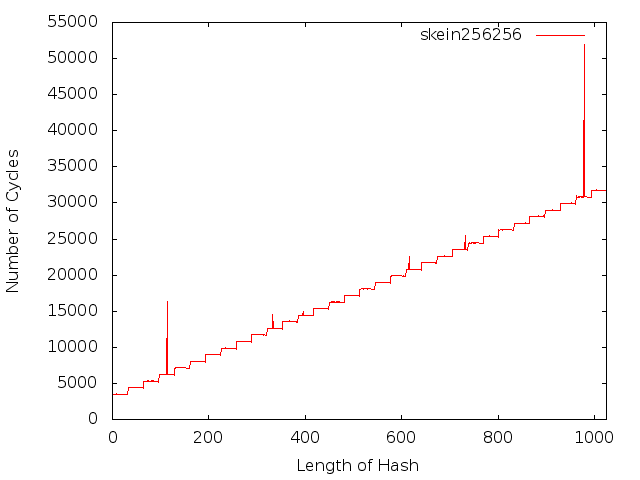
\includegraphics[scale=0.5]{images/skein256256.png} 
            \caption{Skein-256 with 256-bit output}
        \end{center}
    \end{figure}

The implementation of skein256256 chosen for benchmarking was arm\_neon
v1.3\_ARM \_Neon\_code. The measurement function was compiled with \texttt{gcc
-mcpu=strongarm110 -O3 -fomit-frame-pointer} using GCC version 4.4.5. This is
optimized assembly code for the Neon intrinsics. 

This instance of the Skein hash function has a block size of 256-bits (32 bytes) and produces a 256-bit digest.  In this instance, the block cipher operates on 32 byte blocks; naturally, with every higher multiple of 32 a new block must be processed, leading the to the step function represented in the graph.  Because the block size is smaller, there are fewer calculations for the block cipher, resulting in shorter runtimes in comparison to the other Skein hash functions.

\subsubsection{skein512256}

    \begin{figure}[H]
        \begin{center}
            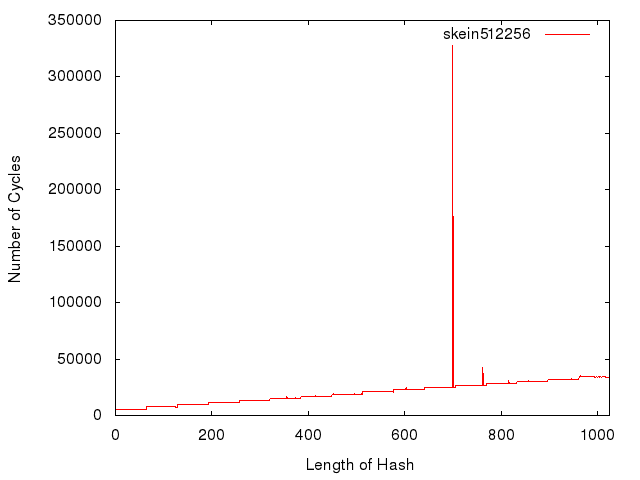
\includegraphics[scale=0.5]{images/skein512256.png} 
            \caption{Skein-512 with 256-bit output}
        \end{center}
    \end{figure}

The implementation of skein512256 chosen for benchmarking was arm
v1.3\_ARM \_assembly\_code and the measurement function was compiled with
\texttt{gcc -mcpu=arm8 -O2 -fomit-frame-pointer} with GCC version 4.4.5.

This instance of the Skein hash function has a block size of 512-bits (64 bytes) and produces a 256-bit digest.  Again, because the block size is 64 bytes, every higher multiple of 64 bytes creates an extra block which must be processed, similar to the previous Skein functions.  The performance of skein512256 is very comparable to the performance of skein256256.  This is because although there are twice as many operations per block in skein512256 (it must handle 64 bytes instead of 32) but there are half as many blocks to process, hence a comparable number of operations must be performed for each algorithm.  The step function is more coarse-grained than skein256256 because of the word size.

\subsubsection{skein512512}

    \begin{figure}[H]
        \begin{center}
            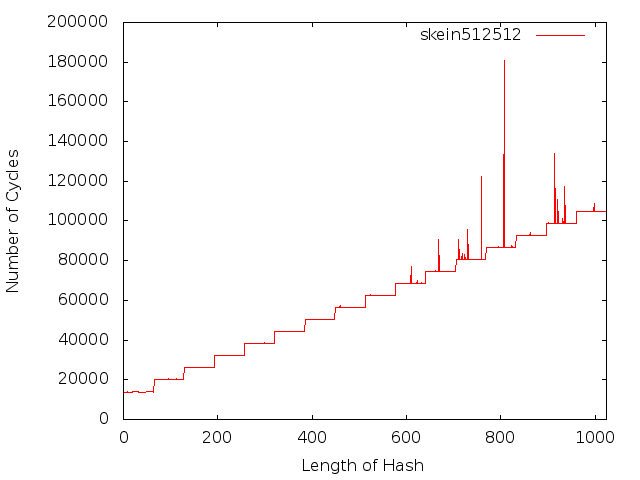
\includegraphics[scale=0.5]{images/skein512512.png} 
            \caption{Skein-512 with 512-bit output}
        \end{center}
    \end{figure}

The implementation of skein512512 chosen for benchmarking was little, compiled
with \texttt{gcc -mcpu=arm920t -O -fomit-frame-pointer} on GCC version 4.4.5.

This instance of the Skein hash function has a block size of 512-bits (64 bytes) and produces a 512-bit digest.  Similar to the other Skein hash funcions, the step size is dictated by the block size; its length is 64 bytes because this instance of the Skein hash function works on 64 byte blocks.  This algorithm shows perfomance slower than skein512256, however - this is because of the output length of the hash.  Skein hash functions use Unique Block Iteration (UBI) chaining to produce the variable size output.  Part of this chaining involves XOR'ing message blocks together with blocks run through the Threefish cipher, and using that output as the input to the next block's chaining.  Because a skein512512 must XOR more words together when chaining the blocks (because the block size is larger), UBI chaining causes performance penalties in comparison to skein512256.

\subsubsection{skein10241024}
    \begin{figure}[H]
        \begin{center}
            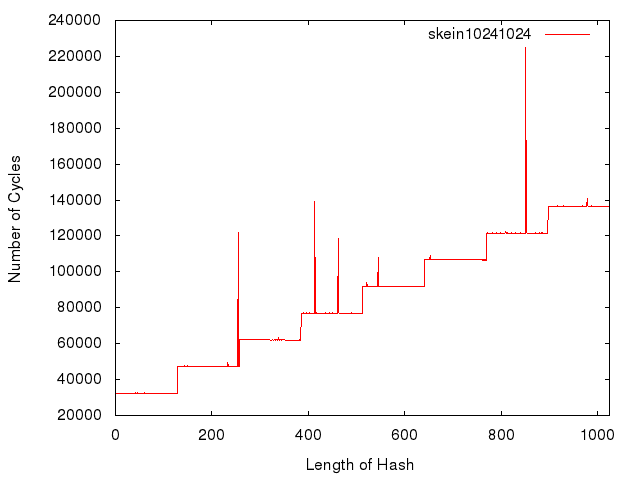
\includegraphics[scale=0.5]{images/skein10241024.png} 
            \caption{Skein-1024 with 1024-bit output}
        \end{center}
    \end{figure}

The implementation of skein10241024 chosen for benchmarking was opt
v1.3\_C\_code which was compiled using \texttt{gcc -O2 -fomit-frame-pointer} on
GCC version 4.4.5.

This instance of the Skein hash function has internal state size of 1024-bits (128 bytes) and produes a 1024-bit digest.  Because the Threefish block cipher works on 128 byte blocks, the step function has a step size of 128 bytes; that is, the number of blocks that must be processed increases with every higher multiple of 128.  Following the analysis for skein512512, this algorithm must also pay a performance penalty for the UBI chaining; it must XOR more words together for each block.  Finally, this implementation has more rounds than other Skein hash functions (80 rounds instead of 72).  Therefore, this implementation has the worst performance of any of the Skein has functions on this architecture.

% CONCLUSION   
%------------
% Contains:
%   - any overall conclusion we can draw from the results of ALL the graphs
%   - lessons learned
\section*{Conclusions}
After running the 25 algorithms over a number of implementations there were several trends. First, the algorithms are in a very optimized state and 
GCC yields little to no improvements. When looking at all of the graphs above another trend that becomes obvious is that the scorpion architecture uses 
32-bit registers. Lastly, there was a stepwise characteristic of each plot depending on the block size or number of blocks in each iteration. These trends
are to be expected given our architecure and the scale of 1-1024 hash sizes.

\bibliography{phase1_bib}{}
\bibliographystyle{plain}
\end{document}
